\documentclass[12pt]{article}
\usepackage{amssymb,mathrsfs, amsmath,amsfonts}
\usepackage{mathtools}
\usepackage{graphicx}
\usepackage{enumitem}
\usepackage{braket}
\graphicspath{ {./ps3-assets/}{./exercises/handwritten/ps3/ps3-assets/} }
%%
%%
\newcommand{\Blank}{\mbox{\hskip 4pt\vrule width 1in depth 2pt}\vrule width 0pt height 2.0em}
\newcommand{\NameBlank}{\mbox{\hskip 4pt\vrule width 2.5in depth 2pt}\vrule width 0pt height 2.0em}
%%
%% Leave at least #1 space, default to what is below
%%
\def\DefaultSpace{1in}
\newcommand{\LeaveSpace}[1][\DefaultSpace]{%
\vskip #1 plus 1fil\relax\hbox to 0pt{\hss} %
}

\title{Problem Set 3}
\author{CSE 468}
\date{\today}

\begin{document}

\maketitle


\noindent Name:\NameBlank{} \newline
\noindent Student ID:\NameBlank{} \newline
\textbf{Note:} You may discuss these problems with other students, but you must write your own solutions.
\begin{enumerate}[font=\bfseries]
    \item (3 points) What is an operation we often use in our circuits that is \underline{not} unitary?
    \item \[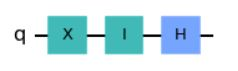
\includegraphics[scale=0.8]{single-q}\]
    (5 points) Describe the above circuit as a single unitary matrix. Show your work.
    \item \[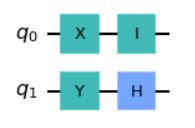
\includegraphics[scale=0.8]{double-q}\]
    (5 points) Describe the above circuit as a single unitary matrix. Show your work.
    \item (3 points) Why would we ever want to consider the tensor product of two gates?
    \item (5 points) Write the below state as the tensor product of two qubits or prove it is an entangled state.
    \[\ket{\psi} = \frac{1}{\sqrt{2}}\ket{00} - \frac{i}{\sqrt{2}}\ket{01}\]
    \item (5 points) Write the below state as the tensor product of two qubits or prove it is an entangled state.
    \[\ket{\psi} = \frac{1}{\sqrt{2}}\ket{01} + \frac{1}{\sqrt{2}}\ket{10}\]
    \item (6 points) Give the statevector of each qubit system.
        \begin{enumerate}
            \item $\ket{10}$
            \item $\ket{0+}$
            \item $\ket{+-}$
        \end{enumerate}
    \item (12 points) Give the parameters ($\theta,\phi,\lambda$) needed for the U gate to specify:
        \begin{enumerate}
            \item the Pauli X gate?
            \item the Pauli Y gate?
            \item the Pauli Z gate?
            \item the Hadamard gate?
        \end{enumerate}
    \item (8 points) Consider the controlled-Y (CY) gate whose behavior is as follows: if the control bit is 0 it does nothing, if the control bit is 1 it applies the Pauli Y gate to the target bit. Give the matrix that describes the CY gate. Could we use this gate to create entanglement? Why or why not?
    \item (10 points) Show the below equality is true.
    \[\frac{1}{\sqrt{2}}(\ket{01} - \ket{10}) = \frac{1}{\sqrt{2}}(\ket{+-} - \ket{-+})\]
    Remember quantum states are equivalent up to a common global phase.
    \item (Bonus, up to 3 points) Write one interesting question related to the content of this homework, and indicate the correct answer. The question can be multiple-choice or free-response.  Interesting questions get credit here;  sufficiently good questions might appear on an exam.
\end{enumerate}



\end{document}